\documentclass[a4paper,11pt,exos]{nsi} % COMPILE WITH DRAFT
\usepackage{pifont}
\usepackage{fontawesome5}
\usepackage{hyperref}

%\usepackage{pgfplots}

%\pgfplotsset{compat=newest}
%\pgfplotsset{every axis/.append style={
%                    axis x line=middle,
%                    axis y line=middle,
%                    axis line style={->},
%                    xlabel={$x$},
%                    ylabel={$y$},
%                    label style={font=\scriptsize},
%                    tick label style={font=\tiny},
%                    unit vector ratio*=1 1 1,
%   					xlabel style={at={(ticklabel* cs:1)},anchor=north west},
%   					ylabel style={at={(ticklabel* cs:1)},anchor=south west}
%                    }}

\begin{document}
\classe{\terminale Comp}
\titre{Fonctions : limites et continuité}
\maketitle

\tabularstyled[UGLiBlue]
\begin{tabular}{p{16.5cm}}
    \rowcolor{UGLiBlue}
    \ths Capacités attendues : \\

    \ding{111} Calculer une fonction dérivée, calculer des limites. Dresser un tableau de variation. \\
    \ding{111} Dans le cadre de la résolution de problème, utiliser le calcul des limites, l’allure des courbes représentatives des fonctions inverse, carré, cube, racine carrée, exponentielle. \\
    \ding{111} Exploiter le tableau de variation pour déterminer le nombre de solutions d’une équation du type $f(x) = k$, pour résoudre une inéquation du type $f(x) \leqslant k$.\\
    \ding{111} Déterminer des valeurs approchées, un encadrement d’une solution d’une équation du type $f(x) = k$.\\
\end{tabular}

\subsection*{Dérivation}

\exo{}
Pour chaque fonction, donner sa dérivée.
\begin{multicols}{2}
    \begin{enumerate}
        \item $f$ définie sur $\R$ par $\quad f(x)=3x^2+2x-5$.
        \item $g$ définie sur $\oio{0}{+\infty}$ par $\quad g(x)=\dfrac{1}{x}+\sqrt{x}$.
        \item 
    \end{enumerate}
\end{multicols}


\dleft{9.5 cm}{
    \exo{}
    $f$ est une fonction dérivable sur $\fif{-5}{6}$. Sa courbe représentative $\mathcal{C}_f$ est donnée dans le repère ci-contre.\\[.5em]
    Lire graphiquement le signe de $f'(x)$ suivant les valeurs de $x$.}
    {\includegraphics[width=6.5cm]{fonction1.jpg}}

\exo{}
Pour chaque fonction, donner sa dérivée.
\begin{multicols}{2}
    \begin{enumerate}
        \item $f$ définie sur $\oio{0}{+\infty}$ par $f(x)=(3x-4)\sqrt{x}$.
        \item $g$ définie sur $\R$ par $g(x)=\dfrac{3x-1}{x^2+1}$.
        \item $h$ définie sur $\R$ par $h(x)=(1-2x)^4$.
        \item $k$ définie sur $\oio{-\dfrac{1}{2}}{+\infty}$ par $k(x)=\sqrt{2x+1}$.
    \end{enumerate}
\end{multicols}

\exo{}
$f$ est la fonction définie sur $\oio{0}{+\infty}$ par $\quad f(x)=x+\dfrac{9}{x}$.
\begin{enumerate}
    \item Déterminer la fonction dérivée de $f$.
    \item Étudier le signe de $f'(x)$ sur $\oio{0}{+\infty}$.
    \item En déduire les variations de la fonction $f$ sur $\oio{0}{+\infty}$.
\end{enumerate}

\subsection*{Fonction exponentielle}
\exo{}
Simplifier au maximum les expressions suivantes.
\begin{multicols}{3}
	\begin{enumerate}[label=\textbullet]
		\item 	$A=e^5\times e^3 \times e^{-4}$
		%\item 	$B=\dfrac{e^7}{e^{-4}}$
		\item	$B=\dfrac{e^{-3}\times e^8}{e^3}$	
		%\item	$D=e^2\times e^{32} \times e^8$
		\item	$C=\dfrac{e}{e^5}$
		%\item	$F=\dfrac{\left(e^7\right)^3\times e^4}{e^{-4}}$
	\end{enumerate}
\end{multicols}

\exo{}
$x$ est un réel quelconque. Simplifier au maximum les expressions suivantes.
\begin{multicols}{3}
	\begin{enumerate}[label=\textbullet]
		\item 	$a(x)=e^{2x}\times \left(e^x\right)^2\times e^{-3x}$
		\item 	$b(x)=\dfrac{e^{x^2}}{e^x}$	
		\item	$c(x)=\dfrac{e^{x-1}\times e^{4x}}{e^x}$
		%\item	$d(x)=\dfrac{e^{-2x}}{e^{-3x}\times e^{x+1}}$
		%\item	$e(x)=\left(e^{4x-5}\times e^{3x+2}\right)^2$
		%\item	$f(x)=\dfrac{e^{3x}}{e^{-x}\times \left(e^{-3x}\right)^2}$
	\end{enumerate}
\end{multicols}


\exo{}
Dans chaque cas, déterminer la fonction dérivée de la fonction définie sur $\R$ par :
\begin{multicols}{3}
    \begin{enumerate}
        \item $f(x)=e^x+x^3$ 
        \item $g(x)=(5x-8)e^x$
        \item $h(x)=\left(3x^2+4\right)\left(1-e^x\right)$
        \item $k(x)=\dfrac{2-e^x}{e^x}$
        \item $l(x)=e^{2x-1}$
        \item $m(x)=2xe^{-x}$
    \end{enumerate}
\end{multicols} 

\exo{}
Résoudre les équations suivantes dans $\R$.
\begin{multicols}{3}
	\begin{enumerate}
		\item	$e^{3x+4}=e^{2x-1}$
		\item 	$e^{x-4}=e$
		\item 	$e^{x^2+x}=1$
		\item	$e^{-x^2}=\dfrac{1}{e}$
		\item	$3+e^x=1$
		\item	$(3x+1)e^x=0$
	\end{enumerate}
\end{multicols}



\begin{minipage}{10cm}
	\exo{}
	On a tracé la représentation graphique d'une fonction $f$ définie sur $\R$. On sait qu'il existe deux réels $a$ et $b$ tels que pour tout $x\in\R, \quad f(x)=(ax+b)e^x$.
	\begin{enumerate}
		\item 	Déterminer graphiquement $f(0)$ et $f(2)$.
		\item 	En déduire la valeur des réels $a$ et $b$.	
	\end{enumerate}
\end{minipage}
\begin{minipage}{1cm}
	\ \\
\end{minipage}
\begin{minipage}{6cm}
	\includegraphics[width=6cm]{courbe1}
\end{minipage}



\exo{}
Résoudre les inéquations suivantes dans $\R$.
\begin{multicols}{3}
	\begin{enumerate}
		\item 	$e^{x+1}<e^4$
		\item 	$e^{-2x+1}\geqslant e^{x-7}$
		\item	$e^{x+1}<1$
		\item	$-3e^{x^2-4}>4$
		\item	$e^{-2x+5}\geqslant 0$
		\item	$e^{x+4}	\leqslant\dfrac{1}{e^{3x}}$
	\end{enumerate}
\end{multicols}

\subsection*{Fonction exponentielle - Démonstrations de cours}
\exo{ Démontrer qu'une expression ne s'annule pas}
On admet qu'il existe une fonction $f$ définie et dérivable sur $\R$ qui vérifie $f(0)=1$ et $f'(x)=f(x)$ pour tout $x\in\R$.\\
On note $g$ la fonction définie sur $\R$ par $g(x)=f(x)\times f(-x)$.
\begin{enumerate}
	\item 	Calculer $g(0)$.
	\item 	Montrer que $g$ est dérivable sur $\R$ et que pour tout $x\in\R, g'(x)=0$.
	\item	Que peut-on en déduire concernant la fonction $g$ ?
	\item	Donner l'expression de $g(x)$ pour tout réel $x$ en utilisant les résultats des questions \textbf{1} et \textbf{3}.
	\item	En utilisant la définition de la fonction $g$, montrer que, pour tout $x\in\R, f(x)\neq 0$.
	\item	\textbf{Bilan :} Que peut-on dire d'une fonction $f$ définie et dérivable sur $\R$ qui vérifie : $f(0)=1$ et $f'=f$.	
\end{enumerate}


\exo{ Démontrer qu'une fonction est unique}
On considère une fonction $f$ définie et dérivable sur $\R$ qui vérifie $f(0)=1$ et $f'(x)=f(x)$ pour tout $x\in\R$.\\
On suppose qu'il existe une deuxième fonction $g$ qui vérifie cette relation : $g(0)=1$ et $g'(x)=g(x)$ pour tout $x\in\R$.\\
On définit également la fonction $h$ sur $\R$ par $h(x)=\dfrac{g(x)}{f(x)}$.
\begin{enumerate}
	\item 	Justifier que $h$ est bien définie.
	\item 	Justifier que $h$ est dérivable sur $\R$ et déterminer sa fonction dérivée.
	\item	En déduire l'expression de $h(x)$ pour tout réel $x$.
	\item	Que peut-on alors en déduire pour les fonctions $f$ et $g$.
	\item	\textbf{Bilan :} \'Enoncer la propriété que l'on vient démontrer pour une fonction $f$ définie et dérivable sur $\R$ et qui vérifie $f(0)=1$ et $f'=f$.
\end{enumerate}



\exo{}
On souhaite démontrer que, pour tous réels $x$ et $y$, $\quad e^{x-y}=\dfrac{e^x}{e^y}$.
\begin{enumerate}
	\item 	\'Ecrire $\dfrac{e^x}{e^y}$ sous la forme d'un produit.
	\item 	Sachant que $e^x\times e^y=e^{x+y}$ et $e^{-x}=\dfrac{1}{e^x}$, démontrer la proposition énoncée.
\end{enumerate}

\subsection*{Limite d'une fonction}

\exo{ Conjecturer la limite d'une fonction en l'infini}
Soient $f$ la fonction définie sur $\R$ par : $\quad f(x)=(x+2)e^{-x}+1\quad$ et $(d)$ la droite d'équation $\quad y=1$.
\begin{enumerate}
	\item \faCalculator\hspace*{.3cm}Tracer sur la calculatrice la courbe représentative de la fonction $f$ et la droite $(d)$ pour $x\in\fif{-3}{3}$ et $y\in\fif{-3}{4}$.
	Que peut-on conjecturer pour les limites de $f$ en $+\infty$ et $-\infty$ ?
	\item Que représente la droite $(d)$ pour la courbe $\mathcal{C}_f$ en $+\infty$ ?
	\item \faPython\hspace*{.3cm}On donne le script Python suivant :\\
	\begin{minipage}{9cm}
		\begin{enumalph}
			\item La fonction \mintinline{python}{abs} revoie la \textbf{valeur absolue} du nombre qui est donné en paramètre.\\[.5em]
			Que renvoit \mintinline{python}{dist(a)} ? 
			\item En exécutant le script, on obtient que \mintinline{python}{dist(10**(-3))} renvoit \mintinline{python}{10} et que \mintinline{python}{dist(10**(-6))} renvoit \mintinline{python}{17}.\\[.5em]
			Qu'est-ce que cela signifie ? 
		\end{enumalph}
	\end{minipage}
	\hspace*{.5cm}
	\begin{minipage}{8cm}
		\begin{pyc}
			\begin{minted}{python}
				from math import *
				def f(x) :
					return (x+2)*exp(-x)+1
				
				def dist(a) :
					x = 1
					while abs(f(x)-1) >= a :
						x = x+1
					return x
			\end{minted}
		\end{pyc}
	\end{minipage}	
\end{enumerate}

\exo{ Conjecturer la limite d'une fonction en un point}
Soit $f$ la fonction définie sur $\R\setminus\{2\}$ par $\quad f(x)= \dfrac{0,5x^2-1,5x+2}{x-2}$.
\begin{enumerate}
	\item \faCalculator\hspace*{.3cm}Tracer sur la calculatrice $\mathcal{C}_f$, la courbe représentative de $f$, dans la fenêtre $x\in\fif{-1}{5}$ et $y\in\fif{-5}{2}$.\\
	Que peut-on conjecturer pour les limites de la fonction $f$ lorsque $x$ tend vers $2$, en valeurs supérieures et en valeurs inférieures ?\\
	Peut-on conjecturer qu'il existe une limite de la fonction $f$ en $2$ ?
	\item Tracer sur le même graphique la droite $(d)$ d'équation $x=2$.\\
	Que représente la droite $(d)$ pour la courbe $\mathcal{C}_f$ en $2$ ?
\end{enumerate}

\exo{  Conjecturer la limite d'une fonction en un point}
Soit $g$ la fonction définie sur $\R^*$ par : $\quad g(x)=\dfrac{e^x-1}{x}$.
\begin{enumerate}
	\item \faCalculator\hspace*{.3cm}Tracer sur la calculatrice $\mathcal{C}_g$, la courbe représentative de $g$, dans la fenêtre $x\in\fif{-4}{4}$ et $y\in\fif{-1}{5}$.
	\item La fonction $g$ est-elle définie en $0$ ? Semble-t-elle admettre une limite finie en $0$ ? Si oui, laquelle ?
\end{enumerate}


\exo{}
On donne ci-dessous la courbe $\mathcal{C}_f$ représentant une fonction $f$.
Dans chaque cas, choisir la ou les bonne(s) réponse(s).\\
\dleft{11.5cm}{
 \begin{enumerate}
	\item La courbe $\mathcal{C}_f$ admet une assymptote verticale d'équation :
	\begin{multicols}{4}
		\begin{enumalph}
			\item $x=-2$
			\item $y=-2$
			\item $x=1$
			\item $y=1$
		\end{enumalph}
	\end{multicols}
	\item La courbe $\mathcal{C}_f$ admet une assymptote horizontale d'équation :
	\begin{multicols}{4}
		\begin{enumalph}
			\item $x=-2$
			\item $y=-2$
			\item $x=1$
			\item $y=1$
		\end{enumalph}
	\end{multicols}
	\item D'après la courbe $\mathcal{C}_f$ on peut dire :
	
 \end{enumerate}
}
{\includegraphics[width=5cm]{courbe1.jpg}}
\begin{multicols}{4}
	\begin{enumalph}
		\item $\lim\limits_{x\to+\infty}f(x)=-2$
		\item $\lim\limits_{x\to-\infty}f(x)=1$
		\item $\lim\limits_{\substack{x \to 1 \\ x>1}}f(x)=+\infty$
		\item $\lim\limits_{\substack{x \to 1 \\ x<1}}f(x)=+\infty$
	\end{enumalph}
\end{multicols}


%\newpage





\subsection*{Opérations sur les limites}

\exo{}
Soit $g$ la fonction définie sur $\R$ par $\quad g(x)=\dfrac{2x^2+3}{4x^2+1}$.
\begin{enumerate}
	\item \faCalculator \hspace*{.3cm} Tracer sur la calculatrice la courbe représentative de la fonction $g$. Que peut-on conjecturer sur les limites de la fonction $f$ en $+\infty$ et en $-\infty$ ?
	\item Vérifier ces conjectures par le calcul.
\end{enumerate}



\exo{}
Soit $h$ la fonction définie sur $\R$ par $\quad h(x)=0,1x^3+0,15x^2-1,8x-0,7$.
\begin{enumerate}
	\item \faCalculator \hspace*{.3cm} Tracer sur la calculatrice la courbe représentative de la fonction $h$. Que peut-on conjecturer sur les limites de la fonction $f$ en $+\infty$ et en $-\infty$ ?
	\item Vérifier ces conjectures par le calcul.
\end{enumerate}


\exo{}
Déterminer les limites en $+\infty$ et $-\infty$ des fonctions suivantes en expliquant la méthode utilisée.
%\begin{multicols}{2}
	\begin{enumerate}
		\item $f$ définie sur $\R$ par $\quad f(x)=x^3-5x^2-x+2$.
		\item $g$ définie sur $\R\setminus \{-1\}$ par $\quad g(x)= 1-x+\dfrac{2}{x+1}$.
		\item $h$ définie sur $\R\setminus\left\{-\sqrt{5}\ ;\ \sqrt{5} \right\}$ par $\quad h(x)=\dfrac{5}{x^2-5}$
		\item $k$ définie sur $\R$ par $\quad k(x)=e^x-2$
	\end{enumerate}
%\end{multicols}

\exo{ Chute libre}
\dleft{11.5cm}{
	La vitesse de chute d'un parachutiste en chute libre, avant qu'il actionne son parachute est modélisée par $$v(t)=50\left(1-e^{-0,2t}\right)$$ 
	où $v(t)$ est la vitesse de chute (en m.s$^{-1}$) du parachutiste en fonction du temps (en secondes).
}
{\includegraphics[width=5cm]{skydiving-297103_1280.png}}
\begin{enumerate}
	\item Quelle est la vitesse du parachutiste à $t=0$ ?
	\item Déterminer $\quad \lim\limits_{t\to +\infty}v(t)$.
	\item Calculer $v'(t)$ pour dresser le tableau de variations de la fonction $v$ sur $\fio{0}{+\infty}$.
	\item Interpréter ce tableau de variations du point de vue du parachutiste.
	\item Dans un article consacré à la découverte du saut en parachute, on peut lire : « Dès la sortie de l'avion et au début du saut, la vitesse de chute augmente très rapidement ; puis la vitesse se stabilise aux alentours de 200 km/h. »\\
	Justifier le propos de cet article.
\end{enumerate}


\exo{}
Pour chaque fonction, déterminer la limite à gauche et à droite de la valeur $a$ donnée, en justifiant le signe du dénominateur.
\begin{enumerate}
	\item $f$ définie par $\quad f(x)=\dfrac{3x-1}{2-x}\quad$ et $\quad a=2$.
	\item $g$ définie par $\quad g(x)=\dfrac{1-2x}{(x+3)^2}\quad$ et $\quad a=-3$.
	\item $h$ définie par $\quad h(x)=\dfrac{e^x}{e^x-1}\quad$ et $\quad a=0$.
	\item $k$ définie par $\quad k(x)=\dfrac{3x^3+1}{x+1}\quad$ et $\quad a=-1$.
\end{enumerate}

\exo{}
$f$ est la fonction définie sur $\fio{0}{+\infty}$ par $\quad f(x)=\sqrt{x^2+1}$.
\begin{enumerate}
	\item Démontrer que pour tout réel $x\geqslant 0, \quad \sqrt{x^2+1}\geqslant \sqrt{x^2}$.
	\item En déduire que pour tout réel $x\geqslant 0, \quad f(x)\geqslant x$.
	\item Étudier alors la limite de $f$ en $+\infty$.
\end{enumerate}


\exo{}
$g$ est la fonction définie sur $\R$ par $\quad g(x)=\dfrac{\sin(x)}{1+x^2}$.
\begin{enumerate}
	\item Montrer que pour tout réel $x : \quad -\dfrac{1}{1+x^2}\leqslant g(x)\leqslant \dfrac{1}{1+x^2}$.
	\item En déduire la limite de $g$ en $+\infty$. Expliquer.
\end{enumerate}


\subsection*{Continuité}

\tabdefault

\exo{ \faCalculator}
$f$ est la fonction définie sur $\R$ par : $\quad f(x)=
\left\{
    \begin{array}{ll}
        -x^2 & \text{si } x<2 \\
        x^2-8 & \text{si } x\geqslant 2 \\
    \end{array}
\right. $
\begin{enumerate}
	\item Afficher, à l'écran de la calculatrice, la courbe représentative de la fonction $f$.\\
	\begin{minipage}{10cm}
		Tutoriel vidéo : \url{https://youtu.be/GWE_ksi9I2c}
	\end{minipage}
	\begin{minipage}{5cm}
		\includegraphics[width=1.7cm]{code-qr1.png}
	\end{minipage}
	\item Conjecturer la continuité de $f$ en 2.
	\item Démontrer cette conjecture.
\end{enumerate}

\exo{ \faPython}
\begin{minipage}{10cm}
	Voici une fonction \mintinline{python}{f} écrite en langage Python.
	\begin{enumerate}
		\item Déterminer l'image par la fonction \mintinline{python}{f} de chacun des nombres suivants :
		\begin{multicols}{5}
			\begin{enumerate}[label=\textbullet]
				\item $0$
				\item $-2$
				\item $5$
				\item $1$
				\item $0,5$
			\end{enumerate}
		\end{multicols}
		\item  Compléter la définition de la fonction $f$ \\[.5em]
		$f(x)=\left\{
			\begin{array}{ll}
				.....\ & \text{si } x<..... \\
				.....\ & \text{si } .....\leqslant x\leqslant ..... \\
				.....\ & \text{si } > .....
			\end{array}
		\right.$
		\item La fonction $f$ est-elle continue sur $\R$ ? Expliquer.
		\item Sur quels intervalles, les plus grands possibles, la fonction $f$ est-elle continue ?
	\end{enumerate}
\end{minipage}
%\begin{minipage}{.5cm}
	\hspace*{.5cm}
%\end{minipage}
\begin{minipage}{6.5cm}
	\begin{pyc}
		\begin{minted}{python}
			from math import*

			def f(x) :
				if x<0 :
					y = exp(x)
				elif x<=1 :
					y = x**2
				else :
					y = 2*x-1
				return y
		\end{minted}
	\end{pyc}
\end{minipage}


\exo{}
$f$ est la fonction définie sur $\R$ par $\quad f(x)=x^4-9x+8$.\\
Démontrer que l'équation $\quad f(x)=5\quad$ admet au moins une solution dans l'intervalle $\fif{-1}{1}$.

\exo{}
$g$ est la fonction définie sur $\R$ par $\quad g(x)=e^x-x^2-5$.\\
Démontrer que l'équation $\quad e^x=x^2+5\quad$ admet au moins une solution dans l'intervalle $\fif{0}{3}$.

\exo{}
$f$ est une fonction continue sur l'intervalle $\fif{-10}{40}$ dont voici le tableau de variations.
\begin{center}
	\begin{tikzpicture}
	\tkzTabInit[color,lgt=3,espcl=2.5]
	{$x$/.7,Variations de $f$ /1.8}
	{$-10$,$21$, $40$}
	\tkzTabVar{-/$-2$,+/$3$,-/$1$}
	\end{tikzpicture}
	\end{center}
\begin{enumerate}
	\item Montrer que l'équation $\quad f(x)=0\quad$ admet une unique solution $\alpha$ dans l'intervalle $\fif{-10}{40}$. 
	\item En déduire le tableau de signes de $f(x)$ dans l'intervalle $\fif{-10}{40}$.
\end{enumerate}

\exo{}
$g$ est la fonction définie sur $\fif{0}{5}$ par $\quad g(x)=xe^x-2e^x-5$.
\begin{enumerate}
	\item Montrer que pour tout réel $x, \quad g'(x)=(x-1)e^x$.
	\item Dresser le tableau de variations de $g$.
	\item Démontrer que l'équation $\quad g(x)=0\quad$ admet une seule solution $\alpha$ dans l'intervalle $\fif{1}{5}$.
	\item Donner un encadrement d'amplitude $1$ de $\alpha$.
\end{enumerate}


\exo{ \faPython \hspace*{.3cm}Méthode de dichotomie}
Le but de cet exercice est de déterminer par une \textbf{méthode de dichotomie} une valeur approchée de la solution de l'équation $\quad x^3+x-1=0$.
\begin{enumerate}
	\item On définit la fonction $f$ sur $\R$ par $\quad f(x)=x^3+x-1$.
	Montrer que l'équation $\ f(x)=0\ $ admet une unique solution $\alpha$ sur $\R$ et que $\alpha\in\fif{0}{1}$.
	\item On veut obtenir un encadrement de $\alpha$. On procède par \textbf{dichotomie} :\\
	On partage l'intervalle $\fif{0}{1}$ en deux intervalles $I_1=\fif{0}{\dfrac{1}{2}}$ et $I_2=\fif{\dfrac{1}{2}}{1}$.
	\begin{enumalph}
		\item Calculer $f\left(\dfrac{1}{2}\right)$.\\
		Expliquer pourquoi $\alpha$ appartient à l'intervalle $I_2$.
		\item On réintère le procédé en partageant l'intervalle $I_2$ en deux : $I_3=\fif{\dfrac{1}{2}}{\dfrac{3}{4}}$ et  $I_4=\fif{\dfrac{3}{4}}{1}$.\\
		Calculer $f\left(\dfrac{3}{4}\right)$.\\
		Dans quel intervalle, $I_3$ ou $I_4$, se trouve $\alpha$ ?
	\end{enumalph}
	\item On automatise ce procédé à l'aide d'un algorithme. On rédige un script Python pour donner un encadrement de $\alpha$ d'amplitude inférieure à $10^{-3}$.
	\begin{multicols}{2}
		\begin{pyc}
			\begin{minted}{python}
				def f(x) :
					return x**3+x-1
				
				def dicho(a,b) :
					n=0
					while b-a >= 10**(-3) :
						c=(a+b)/2
						if f(a)*f(c)<0 :
							b=c
						else :
							a=c
						n=n+1
					return a,b,n
			\end{minted}
		\end{pyc}

		\begin{enumalph}
			\item Que représentent les paramètres \mintinline{python}{a} et \mintinline{python}{b} de la fonction \mintinline{python}{dicho} ?
			\item Quelles valeurs peut-on utiliser pour \mintinline{python}{a} et \mintinline{python}{b} lorsqu'on demande à exécuter la fonction \mintinline{python}{dicho} pour approcher la solution de l'équation $f(x)=0$ ?
			\item Que représente la variable \mintinline{python}{n} ?
			\item Expliquer les quatre lignes d'instructions à partir de \mintinline{python}{if f(a)*f(c)<0 :} 
			\item Utiliser ce programme pour donner un encadrement à $10^{-3}$ de $\alpha$.\\
			En combien d'itération est-il obtenu ?
			\item Que faut-il modifier pour avoir un endrement de $\alpha$ à $10^{-6}$ ?\\
			Donner alors cet encadrement ainsi que le nombre d'itérations nécessaires.
		\end{enumalph}

		
	\end{multicols}
	
\end{enumerate}

\exo{ Bénéfice}
\dleft{11.5cm}{
	Une entreprise est spécialisée dans la production et la vente de peinture éco-responsable.\\
	La production quotidienne varie entre 0 et 800 litres.\\
	Toute la production est vendue. Les montants de la recette et du coût sont exprimés en dizaine d'euros.
}
{\includegraphics[width=5cm]{trend-color-3998738_1280.jpg}}
\begin{enumerate}
	\item Le graphique ci-dessous modélise les recettes et les coûts de production de l'entreprise.\\[.5em]
	\dleft{6cm}{
		\includegraphics[width=6cm]{graphique1.jpg}
	}
	{
		\begin{enumalph}
			\item Que représentent les abscisses sur le graphique ?
			\item Que représentent les ordonnées ?
		\end{enumalph}
	}
	\item A l'aide du graphique, déterminer à partir de quel volume de peinture vendu l'entreprise réalise un bénéfice.
	\item Le bénéfice en dizaine d'euros correspondant à la vente de $x$ centaines de litres de peinture est donné par $\quad f(x)= 25x-150 e^{-0,5x+1}$.\\
	On définit ainsi la fonction $f$ sur l'intervalle $\fif{0}{8}$.
	\begin{enumalph}
		\item Donner les valeurs exactes de $f(0)$ et de $f(8)$, puis en donner les valeurs arrondies au centième.
		\item Montrer que pour tout $x\in \fif{0}{8}, \quad f'(x)=25+75e^{-0,5x+1}$.
		\item Déterminer le signe de $f'(x)$ et en déduire les variations de $f$ sur $\fif{0}{8}$.
		\item Justifier que l'équation $\ f(x)=0\ $ admet une unique solution $\alpha$ sur l'intervalle $\fif{0}{8}$ puis en donner la valeur arrondie au centième.
		\item \faCalculator\hspace*{.3cm}Donner une valeur de $\alpha$ à $10^{-3}$ près. Expliquer la méthode utilisée.
		\item En déduire la quantité de peinture produite et vendue à partir de laquelle l'entreprise réalisera un bénéfice. Donner le résultat au litre près.
	\end{enumalph}
\end{enumerate}




\exo{ Population de grenouilles}
\dleft{11.5cm}{
	Des biologistes étudient l'évolution d'une population de grenouilles autour d'un étang. Ils estiment que le nombre de grenouilles peut être modélisé par : $$P(t)= \dfrac{1000}{0,4+3,6e^{-0,5t}}$$ 
	où $t$ est le temps écoulé (en années) depuis le 1$^{\text{er}}$ janvier 2020.
}
{
	\includegraphics[width=5cm]{tree-frog-474949_1280.jpg}\\
	\centering \footnotesize Grenouille arboricole
}
\begin{enumerate}
	\item Étudier les variations de la fonction $P$ sur $\fio{0}{+\infty}$.
	\item Déterminer la limite de la fonction $P$ en $+\infty$.
	\item Montrer qu'il existe une unique valeur $t_0\in\fio{0}{+\infty}$ telle que $P(t_0)=2000$. \\
	Déterminer cette valeur à $10^{-1}$ près.
	\item  Selon ce modèle, déterminer l'année au cours de laquelle la population dépassera pour la première fois 2000 grenouilles.
\end{enumerate}

\subsection*{Prolongements}

\exo{ Démontrer avec un contre-exemple}
Toutes les propositions suivantes sont fausses. Infimer chacune d'elles à l'aide d'un contre exemple (qui peut être graphique).
\begin{enumerate}
	\item $f$ est une fonction définie sur $\R$ telle que : $\quad \lim\limits_{x\to-\infty}f(x)=-\infty\quad$ et $\quad \lim\limits_{x\to+\infty}f(x)=+\infty$\\
	donc $f$ est croissante sur $\R$.
	\item $f$ est une fonction strictement croissante sur $\R$ donc $\quad \lim\limits_{x\to+\infty}f(x)=+\infty$.
	\item $f$ est une fonction définie sur $\fio{0}{+\infty}$ telle que $\ f(0)=0\ $ et $\ \lim\limits_{x\to+\infty}f(x)=+\infty\ $ donc $f$ est positive sur $\R$.
	\item Si $f$ est une fonction définie sur l'intervalle $\fif{-1}{2}$, alors $f$ est continue sur l'intervalle $\fif{-1}{2}$.
	\item Si $f$ est une fonction continue sur l'intervalle $\fif{-1}{2}$ telle que $\ f(-1)=-2\ $ et $\ f(2)=3, \ $ alors l'équation $\ f(x)=0\ $ admet une unique solution dans l'intervalle $\fif{-1}{2}$.
\end{enumerate}


\exo{}
$f$ est la fonction définie sur $\R$ par $\quad f(x)=\dfrac{x^4}{4}-\dfrac{3}{2}x^2+4x$.
\begin{enumerate}
	\item Déterminer l'expression de $f'$, la fonction dérivée de $f$ et de la fonction dérivée de $f'$, notée $f''$ (dérivée seconde de $f$).
	\item \begin{enumalph}
		\item Étudier les variations de la fonction $f'$.
		\item Dresser le tableau de variations de $f'$ et en déduire que l'équation $\ f'(x)=0\ $ admet une unique solution $\alpha$ dans l'intervalle $\oif{-\infty}{-1}$.
		\item \faCalculator\hspace*{.3cm}Donner un encadrement d'amplitude $10^{-2}$ de $\alpha$.
	\end{enumalph}
	\item \begin{enumalph}
		\item Déterminer le signe de la fonction $f'$.
		\item Dresser le tableau de variations de la fonction $f$.
		\item Montrer que $\ f(\alpha)=\dfrac{3}{4}\alpha(4-\alpha)$.
		\item Déterminer le nombre de racines du polynôme $f$.
		
	\end{enumalph}
\end{enumerate}

\end{document}